%%
% E = mc^2 - Book & Chapter Summary, for the English cuurse "Where Tech Meets BEC".
%
% (C) 2016 by Nikola Stankovic, University of Applied Sciences Rapperswil
%%

\documentclass[a4paper,12pt]{scrreprt}

%% Load packages
%% ========

\usepackage[T1]{fontenc}
\usepackage[utf8]{inputenc}
\usepackage{lmodern}
\usepackage[english]{babel}
\usepackage[]{setspace}
\usepackage{amsmath}
\usepackage{amssymb}
\usepackage{geometry}

\geometry{papersize={210mm,297mm},total={160mm,240mm},top=31mm,bindingoffset=15mm}

%% Own variables
%% ========
\newcommand{\documentauthors}{Nikola Stanković, Robin Suter, Jonas Matter, Marcel Stocker, Patrick Scherler}
\newcommand{\documenttitel}{E = mc$^2$}
\newcommand{\documentsubtitel}{Book \& Chapter Summary}

%% PDF meta informations
%% ========
\pdfinfo{
   /Author (\documentauthors)
   /Title  (\documenttitel)
   /CreationDate (D:20040502195600)
   /Subject (English, Where Tech Meets BEC)
   /Keywords (English;BEC;HSR)
}

\begin{document}
\author{\documentauthors \\ University of Applied Sciences Rapperswil \\ St. Gallen, Switzerland}

\title{\documenttitel}
\subtitle{\documentsubtitel}
\maketitle
\tableofcontents

%% All content of this work
%%
% context.tex
%
% @author: Nikola Stankovic
%%

\chapter{Context}
more is coming soon :) ...

%%
% summary.tex
%
% @author: Nikola Stankovic
%%

\chapter{Summary}
more is coming soon :) ...

%%
% character-list.tex
%
% @author: Nikola Stankovic
%%

\chapter{Character List}
more is coming soon :) ...

%%
% analysis-of-major-character.tex
%
% @author: Nikola Stankovic
%%

\chapter{Analysis of Major Character}
more is coming soon :)  ...

%%
% themes-motifs-and-symbols.tex
%
% @author: Nikola Stankovic
%%

\chapter{Themes, Motifs, and Symbols}
more is coming soon :) ...

%%
% summary-and-analysis.tex
%
% @author: Nikola Stankovic
%%

\chapter{Summary and Analysis}

%%
% Chapter_Bern-Patemt-Office-1905.tex
%
% @author: Nikola Stankovic
%%

\section{Bern Patent Office, 1905}

\emph{Hermann Einstein}, Albert Einstein's father, wrote to \emph{Professor Wilhelm Osterwald} to please him to write a letter to Albert with a few words of encouragement, so that be might recover the joy of Einstein in living and working. Einstein felt profoundly unhappy with his lack of position in that time and his idea that he has gone off the tracks with his career. No answer from Professor Osterwald was ever received.

In the year 1905, Einstein wrote a series of papers that changed our view of the universe forever.

Einstein married a fellow student, \emph{Mileva}, and worked in the patent office. He spent his time often in pub visits and long walks. Einstein's final university grades were unusually low. Teachers were irritated by his lack of obedience. Everyone in authority seemed to enjoy putting Einstein down.

Einstein and his wife had given away their first child, a daughter born before they were married. He couldn't even afford the money for part-time help to let his wife go back to her studies.

Even the hours he had to keep at the patent office worked against him. By the time he got off for the day, the one science library in Bern was usually closed. During the few free moments, he scribbled on sheets he kept in one drawer of his desk - which he jokingly called his "department of theoretical physics".

The first articles he wrote weren't especially impressive. He was always aiming for grand linkages

Einstein wrote his theory of relativity in just five or six weeks filling thirty-some pages. He sent his articles to \emph{Annalen der Physik} to be published. A few weeks later he realized that he had left something out, so he delivered a supplement.
%%
% E-is-for-Energy.tex
%
% @author: Nikola Stankovic
%%

\section{E is for Energy}
More coming soon ...
%%
% equalsymbol.tex
%
% @author: Nikola Stankovic
%%

\section{=}
%%
% m-is-for-mass.tex
%
% @author: Nikola Stankovic
%%

\section{m is for mass}
%%
% quiet-in-the-midday-snow.tex
%
% @author: Robin Suter
%%

\section{Quiet in the Midday Snow}

%%
% germanys turn.tex
%
% @author: Robin Suter
%%

\section{Quiet in the Midday Snow}

%%
% norway.tex
%
% @author: Robin Suter
%%

\section{Norway}

%%
% 13_0816-am-over-japan.tex
%
% @author: Jonas Matter
%%

\section{8:16 A.M. - Over Japan}

%%
% 14_the-fires-of-the-sun.tex
%
% @author: Jonas Matter
%%

\section{The Fires of the Sun}

%%
% 16_a-brahmin-lifts-his-eyes-unto-the-sky.tex
%
% @author: Jonas Matter
%%

\section{A Brahmin Lifts His Eyes Unto the Sky}


more is coming soon :) ...

%%
% study-questions.tex
%
% @author: Nikola Stankovic
%%

\chapter{Study Questions}

\subsection*{Questions for the preface}
\begin{enumerate}  
\item What is the book about?  
\item What is NOT the topic of the book?
\item Why is there a central section about WW2?
\end{enumerate}

\subsection*{Questions for part 1}
\begin{enumerate}  
\item What was Einstein’s economic and family situation around 1900-1905? 
\item How well did Einstein do in his final physics university exams?
\item Where did Einstein do his research?
\item Where exactly did Einstein publish his ground-breaking formula?
\end{enumerate}

\subsection*{Questions for part 2}
\subsubsection*{E is for Energy}
\begin{enumerate}  
\item What kind of apprenticeship did Michael Faraday make?
\item How did he get in touch with Humphrey Davy?
\item What was the relationship between Humphrey Davy and Michael Faraday like?
\item How much formal education did Faraday have?
\item What explains Faraday’s ability to understand the connection between magnetism and electricity?
\item What is this? And when was it built? \\
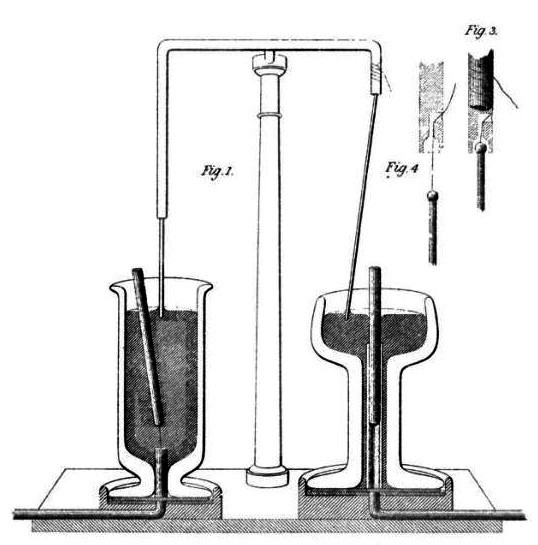
\includegraphics[width=0.5\textwidth]{images/image-part-1-question-6.jpg}\par\vspace{1cm}
\item What does the Law of the Conservation of Energy mean?
\item What new energy source did Einstein discover and what effect does this have on the Law of the Conversion of Energy?
\end{enumerate}

\subsubsection*{=}
\begin{enumerate}  
\item When were most typographical symbols created?
\item How did Einstein use the = symbol ‘like a telescope’?
\end{enumerate}

\subsubsection*{m is for Mass}
\begin{enumerate}  
\item How is Lavoisier’s character described?
\item What did Lavoisier discover when analysing the burning/rusting of metals?
\item Which famous scientist had already developed a theory of mass and movement in the 1600s?
\item Why was Lavoisier so unpopular during the French revolution?
\item What was Einstein taught in the 1890s about mass and energy?
\item How did Einstein establish a link between the two domains?
\end{enumerate}

\subsubsection*{c is for Celeritas}
\begin{enumerate}  
\item Who was the first scientist to try to measure the speed of light?
\item How did Ole Roemer discover the speed of light?
\item What is the explanation given for the fact that Roemer discovered the speed of light?
\item How did Cassini react to Roemer’s success?
\item How fast is the speed of light?
\item In what ways were Faraday and Maxwell similar?
\item What is the inner property of light?
\item In what ways is light different from other movement?
\item Why is it impossible to catch up with the speed of light?
\item Why is -273${^\circ}$ the coldest possible temperature?
\item What happens to matter approaching the speed of light?
\item ''Energy does not stand alone, and neither does mass. But the sum of ? will always remain constant.'' What is in the gap?
\item Why did nobody before Einstein notice the connection between mass and energy?
\end{enumerate}

\subsubsection*{To the power of 2}
\begin{enumerate}  
\item Who was Voltaire?
\item What was Emilie du Châtelet like? 
\item What was the dispute between Leibniz and Newton about?
\item Why was this also a religious conflict?
\item How did du Châtelet prove that Leibniz was right?
\item Why is squaring the velocity of what you measure such an accurate way to describe what happens in nature?
\item What does it mean for mass when c2 is such a large figure?
\item Mass is simply the ultimate type of condensed or concentrated ?
\end{enumerate}

Listen to some of the 10 scientists explaining E = mc$^2$ to help you further your understanding of the formula! \url{http://www.pbs.org/wgbh/nova/einstein/experts.html}

\subsection*{Part 3}
\subsubsection*{Einstein and the equation}
\begin{enumerate}  
\item When and where did Einstein publish the equation?
\item What material discovered in the 1890s gave hints about the equation?
\item Who was Marie Curie and how did she die?
\item Why are atomic bombs so powerful?
\item What was so ground-breaking and amazing about Einstein’s discovery? (p. 80, 84)
\item How precisely did he discover it? (p. 80 top)
\item How could you explain the theory of relativity easily? (p. 83)
\item What does the term ‘relativity’ NOT mean? (p. 84)
\item How did Einstein’s upbringing and background help him discover ‘relativity’?
\item How did Einstein’s family life develop as his theory became gradually accepted?
\end{enumerate}

\subsubsection*{Into the atom}
\begin{enumerate}  
\item How is Ernest Rutherford’s character described?
\item What break-through discovery about the atom did he make? 
\item Why did scientists assume that a lot of energy was hidden in the nucleus?
\item Who was James Chadwick and what did he discover?
\item Who was Enrico Fermi?
\item What important technique did he provide in 1934?
\end{enumerate}

\subsubsection*{Quiet in the midday sun}
\begin{enumerate}  
\item Who were Lise Meitner and Otto Hahn?
\item What happened to Hahn and Meitner’s work in 1938?
\item When did Meitner first meet Einstein and what did she learn there?
\item How did Meitner manage to explain the Meitner-Hahn-Strassmann experiments in 1938?
\end{enumerate}

\subsection*{Part 4}
\subsubsection*{Germany’s turn}
\begin{enumerate}  
\item Why did Einstein write a letter to the American president in 1939 and what was the reply?
\item Why did the USA not pursue plans to build a bomb, while the Germans did?
\item Who was Heisenberg and why did he get in trouble with the SS?
\item What saved him?
\item What was Heisenberg’s bomb design based on?
\item What happened at Heisenberg’s first test in early 1941?
\item How did the Germans produce Uranium dust?
\item When did the Germans get the first successful test results?
\item When did the Americans start to develop their bomb and what was the name of the project?
\item What was superior about the American bomb design?
\item What did the Allied forces do to win the race for the bomb?
\end{enumerate}

\subsubsection*{Norway}
\begin{enumerate}  
\item How did the Allied forces try to sabotage the German bomb project?
\item What happened in the first attack on the Norwegian plant? 
\item What was different in the second sabotage attempt?
\end{enumerate}

\subsubsection*{America’s turn}
\begin{enumerate}  
\item Who was appointed as the day-to-day manager of the Los Alamos bomb construction team?
\item What was Oppenheimer like and how did he motivate his team? 
\item Which two ways to build a bomb did America pursue?
\item How did the scientists try to make Plutonium explode?
\item What news did Niels Bohr bring from Europe in February 1944?
\item What kind of sabotage did the Norwegian Haukelid do?
\item What did finally happen to Germany’s bomb building capacity?
\item What happened to Heisenberg?
\item What happened to Oppenheimer after the war?
\item Which two opposing views were there in the US concerning the deployment of the bomb in Japan?
\item Why was the bomb deployed?
\end{enumerate}

\subsubsection*{8:16 A.M. – Over Japan}
\begin{enumerate}  
\item What happened inside the bomb when it was triggered?
\item Why was it triggered at 2000 ft. above ground? 
\item What is the condition inside the triggered bomb compared to?
\item How much heat is produced?
\item What happens on the ground?
\end{enumerate}

\newpage
\subsection*{Part 5}
\subsubsection*{The fires of the sun}
\begin{enumerate}  
\item What is the topic of this chapter? (p. 173)
\item What did astronomers believe about the sun’s content at the time Einstein discovered that E=mc2? 
\item How does a spectroscope work?
\item What was Cecilia Payne’s academic career?
\item How did Payne come up with a different interpretation of the spectroscope lines?
\item How did the astronomy establishment react to her findings?
\item What happens inside the sun to release so much energy?
\end{enumerate}

\subsubsection*{Creating the earth}
\begin{enumerate}  
\item What is the leading question of this chapter? (p. 185)
\item How did Hoyle explain the creation of the elements? 
\item Where did he get his inspiration for the theory of implosion?
\item What keeps our planet hot at the core and causes continental shifts (earthquakes)?
\item What examples of modern human applications of E=mc2 are given?
\end{enumerate}

\subsubsection*{A Brahmin lifts his eyes unto the sky}
\begin{enumerate}  
\item What will happen to the sun in five billion years?
\item What concept did Chandra come up with on a trip from India to England in 1930? 
\item What will happen to planet Earth in six billion years?
\end{enumerate}





\end{document}